%Author Alex Clemmer
%CS 3100 Computer Organization
%Assignment 6:
\documentclass[a4paper]{article}
\usepackage[pdftex]{graphicx}
\usepackage{fancyvrb}
\usepackage{multirow}
\usepackage{amssymb}
\usepackage{amsmath}
\usepackage{haldefs}

\begin{document}

\section*{Assignment 6 }
Alex Clemmer\\
Student number: u0458675

\subsection*{Problem 1:} 

\paragraph{Running the buggy program:} See the typescript $\texttt{yacc-buggy-script}$.

\paragraph{With fixed associativity:} See the typescript $\texttt{yacc-corrected-script}$.

\paragraph{Calculator, rewritten:} See $\texttt{page58-expr.y}$ for the yacc file (for problem $\textbf{1 a)}$). For the typescript (problem $\textbf{1 b)}$), see the file $\texttt{page-58-expr.y}$.

\paragraph{Evaluating expressions:} See file \texttt{fullcalc-script} for execution and explanations.

\paragraph{Evaluation of complex expressions:} See file \texttt{fullcalc-script} for execution and explanations.

\subsection*{Problem 2:} 

\begin{verbatim}
S -> A | B | C
A -> 0A | 11A | 2B
B -> A0 | B2
E -> 0C | 2D
C -> 0C | 1S | 3A | 4
\end{verbatim}

First eliminate  $\texttt{E}$ because it is not mentioned in any other rules.

\begin{verbatim}
S -> A | B | C
A -> 0A | 11A | 2B
B -> A0 | B2
C -> 0C | 1S | 3A | 4
\end{verbatim}

Neither $\texttt{B}$ nor $\texttt{A}$ actually ever generate anything. Eliminate them.

\begin{verbatim}
S -> C
C -> 0C | 1S | 4
\end{verbatim}

At this point, $\texttt{S}$ generates only $\texttt{C}$. Thus we can combine them.

\begin{verbatim}
S -> 0S | 1S | 4
\end{verbatim}

\subsection*{Problem 3:} 

\begin{verbatim}
S -> S01 | P23 | R4 | 7
R -> S5 | P5 | 6
P -> P8 | 9
\end{verbatim}

To reverse a grammar, we simply reverse each individual production rule. This proof is actually sort of fascinating: for some language $L$ we have some string $z \in L$. Say $z = pqr : |p|, |q|, |r| \geq 0$. Let us consider the simplest case, $\textit{i.e.}$, that each of $p$, $q$, and $r$ is generated by one and only one rule that produces $\textit{only}$ terminals (for example $\texttt{A -> 01}$, rather than $\texttt{A -> TB}$ [or something else with variables]).

The way to reverse a string by components is as follows (anything else yields incorrect results): $(xyz)^R = x^R y^R z^R$, so we can describe the reverse of $z$ as $z^R = r^R q^R p^R$. Since we are considering the case where the production rule of $p$, $q$, and $r$ is $\textit{only}$ terminals (and hence, not variables), each of these has a straightforward reversal, $\textit{e.g.}$, $\texttt{A-> 01}$ will become $\texttt{A-> 10}$.

Now, considering the example where each production rule for $p$, $q$, and $r$ may have variables, the case is not different. Each production rule, even those with variables, must by definition eventually lead to some set of terminals (otherwise it's a non-generating rule), so we can reduce a string like $pqr$ to this more complicated case by considering, for example, that $p$ might be defined with more variables, $\textit{e.g.}$, $wt$.

If $w$ and $t$ both are both production rules that generate $\textit{only}$ terminals, we can reverse $p$ by reversing both of them individually, and then reversing their order. This proves that the above principle holds for any production rule that pertains purely to terminals, AND can be extended to hold for $\textit{any}$ production rule that is nested above a production rule that results directly in terminals. Since all production rules are contained in some path that ends in terminals, this holds for all CFGs.

Thus, the reversed version of the above grammar is:

\begin{verbatim}
S -> 10S | 32P | 4R | 7
R -> 5S | 5P | 6
P -> 8P | 9
\end{verbatim}

The NFA is as follows: \\
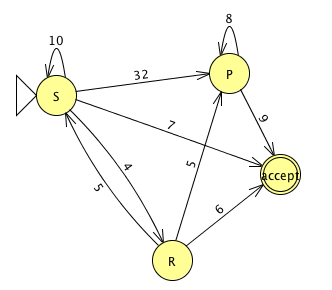
\includegraphics[width=100mm]{3_nfa.png}

\subsection*{Problem 4:}

Given the language $L = \{ww | w \in \{0,1\}^*\}$ and the string $z = 0^n 1^n 0^n 1^n$. $z$ can be split as $z = uvwxy$. Let us consider the following cases:

\paragraph{a)} When $v$ and $x$ fall within first $0^n$, then $vwx$ must clearly consist of at most one $\textit{type}$ of character (which in this case is $0$). When we pump $v$ and $x$, then we end up adding more $0$s. In order for this to still be a part of the $L$, we would have to add corresponding $1$s and $0$s in the other places where there are $n$ repetitions of that character ($\textit{e.g.}$, for string $0^n 1^n 0^n 1^n$, we'd have to add a $1$, a $0$, and a $1$ to each respective repetition after the first $0^n$).

\paragraph{b)} In the case where $v$ falls within the first $0^n$ and $x$ falls within the first $1^n$, we $\textit{still}$ can't pump. $vwx$ would consist of at most two types of characters (in this case, we're told that it consists of $0$ and $1$); when we pump $v$ and $x$, we end up with $i$ more $0$s and $1$s in the first half, but the second half remains the same. In other words, if we had the string $00110011$, and we pumped just once given the above assumptions, we could have $0001110011$, which is $\textit{clearly}$ not inside $L$.

\paragraph{c)} In the case where $v$ falls within the first $1^n$ and $x$ falls within the second $0^n$, we would have a similar result as the two above. In short, pumping would yield more characters in both the first set of $1$s and the second set of $0$s, which leaves the first set of $0$s and the second set of $1$s with $n$ repetitions, where the other two sets have $n + i : i \in \mathbb{Z}$ repetitions. So clearly this string would not be in $L$.

\paragraph{d)} There are a couple of cases we could (and should) consider here: (1) any time $v$ and $x$ fall in the same symbol space ($\textit{e.g.}$, they both fall within the first $0^n$, or the last $1^n$); (2) any time they end up in different symbol spaces ($\textit{e.g.}$, one falls in the first $0^n$, the other falls in the second $0^n$); (3) any time $x$ or $v$ straddles more than one of the symbol spaces ($\textit{e.g.}$, $x$ takes up the first $0^n$ as well as the first $1^n$).

There are various permutations of this that can be considered (that is, there are multiple situations that satisfy each rule), but it would probably be sufficient to show that there is a systematic problem with each of them. For example, you could show pretty easily that any time you pump one or more types of symbol, the string is no longer in $L$, because you simply can't pump ALL the types of symbol in the given string $z$; you have to pick 1, 2, or maybe even 3 out of the 4, and that $\textit{always}$ violates $L$.

\subsection*{Problem 5:}

$\texttt{If-then-else}$ ambiguity occurs when there are two $\texttt{if-then}$ structures do the exact same thing, except for one important difference: one has an $\texttt{else}$ clause that sends the user down a different logic path. This is very bad, because the user may arbitrarily be sent down the $\texttt{else}$ path, or not. When constructing anything that needs to deal with data reliably, obviously we don't want this sort of thing to be ambiguous; we want to always know what will happen.

The modified grammar is as follows:

\begin{verbatim}
STMT -> MATCHED | UNMATCHED
MATCHED -> if EXPR then MATCHED else MATCHED | OTHER
UNMATCHED -> if EXPR then STMT
           | if EXPR then MATCHED else UNMATCHED
OTHER -> p
EXPR -> q
\end{verbatim}

The ambiguity here is clearly eliminated simply because there is no way for a user to be arbitrarily sent down some $\texttt{else}$ path. These instructions are clear and unambiguous: the $\texttt{else}$ is always bound to the closest $\texttt{then}$.

\subsection*{Problem 6:} 

\paragraph{a)} $X$ is nullable because it directly produces $\varepsilon$; $Y$ is a bit subtler, but it can call $X$ directly, $\textit{i.e.}$, with no terminals around it, and can therefore also produce $\varepsilon$.

\paragraph{b)} We eliminated $\varepsilon$ (rule 1), and then we eliminated the production $Y \to X$ (rule 2). Doing that last step, at least in this case, is pretty simple: since $Y \to X$ with literally no terminals or complications around the invocation of $X$, we are able to just put everything in $X$ as a production of $Y$. Note that we also retain $Y$'s only unique production, the terminal $c$.

\paragraph{c)} The derivation sequence for $\texttt{ab}$ is as follows: $\texttt{S -> AB -> ab}$. The derivation sequence for $\texttt{abbb}$ is $\texttt{S -> EF -> AXBX -> aXBX -> aXbX -> abbX -> abbb}$.

\subsection*{Problem 7:} 

The following is the PDA for example 9.2 on page 84. Note that I did the Chomsky Normalized form; the PDA for the original is a lot simpler (but who doesn't like a challenge?):\\
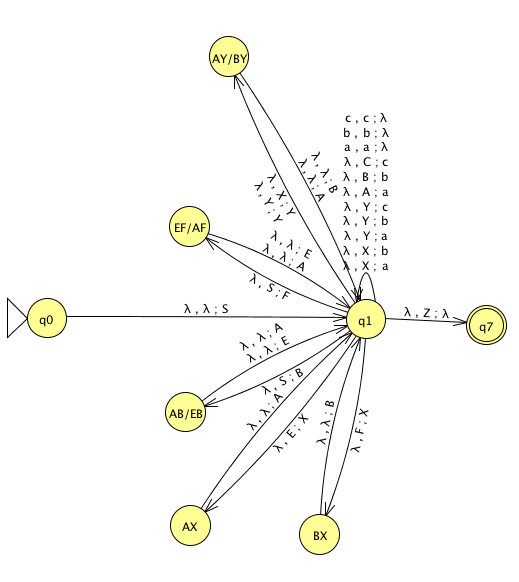
\includegraphics[width=110mm]{7_pda.png}

And these are the results of some of the strings I fed it:\\
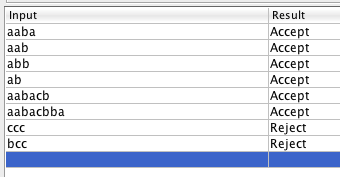
\includegraphics[width=80mm]{7_results.png}


\subsection*{Problem 8:} 

The PDA state $\texttt{A=[p,Z0,p]}$ actually implies a couple of rules, but the one we are concerned with comes from comes from the second rule of the PDA: $\texttt{[p,Z0,r\_2] ->}$ $\texttt{( [p,(,r\_1] [r\_1,Z0,r\_2] for r\_i in \{p,q\} }$. This comes from the last general rule in the text: "General rule: If ?(p,a,g) contains ?q,g1,...,gn, introduce one generic rule [p,g,q0] $\to$ a [q,a,q1][q1,g1,q2]...[qn,gn,q0]
 and create one instance of the rule for each qi $\in$ Q chosen in all possible ways." In fact, this is nearly a one-to-one mapping for the rule generated.


\end{document}